\section{Evaluation}
\label{sec:evaluation}

We prove the correctness and liveness of \sys in Appendix~\ref{appx:hierarchical_merge}.
Our evaluation centers around four aspects:

\parab{Efficiency.} First, \sys achieves low reordering delay, which is the delay from receiving to delivering a packet. With beacon interval of 100$\mu$s, we achieve 

\parab{Scalability.}

\parab{Fault tolerance.}

\parab{Real-world application.}

we first evaluate the reordering delay, CPU overhead and network overhead of \sys under normal conditions.
Then we deep dive into the behavior of \sys under packet loss, failure and incremental deployment.

\subsection{Methodology}
\label{sec:testbed}

We build two testbeds in two data centers.
The first one has 3 servers connected to a Barefoot Tofino 100G switch~\cite{tofino}.
The second one has 32 servers and 10 Arista 7060CX 100G switches~\cite{arista}, forming a fat-tree topology.
Each server has two Xeon E5 CPUs and one Mellanox ConnectX-4 NIC running RoCEv2~\cite{infinibandrocev2}.

%We use a testbed of 8 Dell R720/R730 servers and 10 Arista 100G Ethernet switches~\cite{arista} to benchmark the efficiency of \sys. %The topology is similar to Figure~\ref{fig:dcn}. 
%Each server is equipped with two Xeon E5 CPUs and one Mellanox ConnectX-4 NIC. Because we have not found a low latency interface in the switch OS to process beacon packets, we connect one Dell R720 server with Mellanox ConnectX-3 NICs to each of the switches to mimic the switch CPU. %Since the bottleneck in our benchmarks is the CPU instead of the network, there is unlikely to be congestion loss.
%Performance using data-plane programmable switches are expected to be better, but not evaluated because we do not have such a switch.

In throughput tests, each server uses 8 send cores and 8 receive cores in parallel.
To minimize inter-core synchronization, each pair of send and receive cores is considered a unique host which maintains timestamps independently and processes unreliable datagrams via a separate RDMA queue pair.

\iffalse
\begin{table}[t]
\centering
\scalebox{0.85}{
\begin{tabular}{|l|r|r|r|r|r|r|}
\hline
Servers & \multicolumn{3}{c|}{Num switches} & \multicolumn{3}{c|}{Num downlinks} \\
\hline
Host & ToR & Leaf & Core & ToR & Leaf & Core \\
\hline
2	 & 1 & 0 & 0 & 2 & 0 & 0 \\
\hline
4    & 2 & 2 & 0 & 2 & 2 & 0 \\
\hline
8    & 4 & 4 & 2 & 2 & 2 & 4 \\
\hline
64    & 8 & 4 & 2 & 8 & 4 & 4 \\
\hline
1024  & 64 & 16 & 8 & 16 & 16 & 16 \\
\hline
\end{tabular}
\vspace{-10pt}
}
\caption{Network topologies for evaluation.}
\label{tab:eval-topology}
\end{table}

We evaluate 5 different system scales in Table~\ref{tab:eval-topology}: testbed consisting of one to three layers of network switches, as well as simulation of three-layer fat-tree topology with 64 or 1024 hosts.
Topologies in Table~\ref{tab:eval-topology}.
For large-scale experiments, we use NS-3~\cite{henderson2008network} for simulation.
The link bandwidth, link delay and processing delay are extracted from three-layer testbed experiments.
To make simulations faster, each sender only sends one message to a randomly chosen receiver.
\fi




\subsection{Efficiency}



\begin{figure}[t]
\centering

\includegraphics[width=0.3\textwidth]{images/fixme.pdf}
\caption{[Testbed] Throughput comparison with hierarchical merge using end hosts only.}
\label{fig:hierarchical-merge}
\end{figure}

Figure~\ref{fig:hierarchical-merge} compares the throughput and latency using P4 programmable switch, commodity switch, end host barrier and hierarchical merge.
\RED{Bojie will fill in the figure.}



\begin{figure}[t]
\centering

\includegraphics[width=0.3\textwidth]{images/fixme.pdf}
\caption{[Testbed] Reordering delay with different clock synchronization methods.}
\label{fig:clock-sync}
\end{figure}

Figure~\ref{fig:clock-sync} compares reordering delay of minimax clock synchronization with physical clock synchronization.
\RED{Bojie will fill in the figure.}


\begin{figure}[t]
\centering
	\subfloat[Process beacon packets with switch CPU or end hosts in 5 system scales.\label{fig:reorder-testbed}]
	{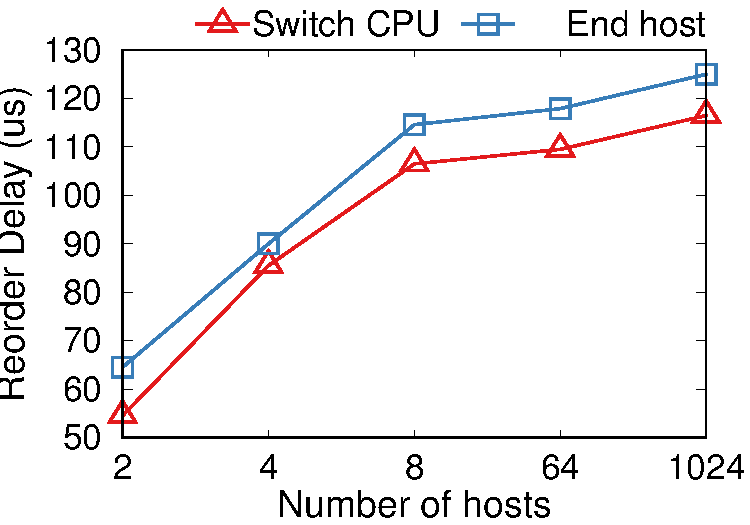
\includegraphics[width=.23\textwidth]{gnuplot/reorder_testbed.pdf}}
	\hspace{0.01\textwidth}
	\subfloat[Simulation with different end-host delays.
	T-R\textit{i} shows minimax clock synchronization, P-R\textit{i} shows physical clock synchronization.\label{fig:reorder-simulation}]
	{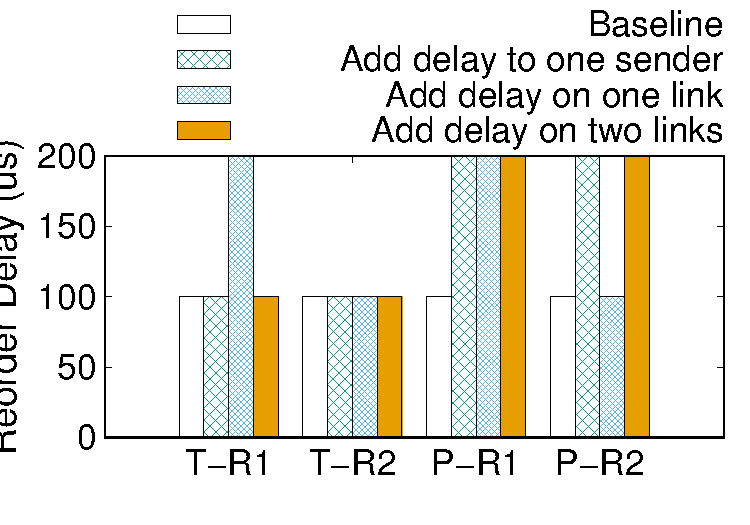
\includegraphics[width=.23\textwidth]{gnuplot/reorder_simulation.pdf}}
	\caption{Average reordering delay. Beacon interval is 100~$\mu$s.}
    \vspace{-5pt}
\label{fig:reorder-delay}
\end{figure}

\subsubsection{Reordering Delay}
\label{sec:eval-delay}

Figure~\ref{fig:reorder-testbed} shows the average reordering delay in different system scales.
Because the beacon interval is 100~$\mu$s, the average reordering delay to wait for the next beacon is 50~$\mu$s.
Using end host representatives to process beacons introduces additional delay due to forwarding delay from the switch to the end host representatives.
As the number of network layers increase, the reordering delay increase, due to beacon processing delay at each switch.
The beacon interval is not amplified by network layers, because the algorithm synchronizes beacon arrival times.
For three-layer topology, the number of hosts adds slightly to reordering delay, because a switch with higher fan-out is likely to have more skew in beacon synchronization.

Figure~\ref{fig:reorder-simulation} compares how minimax clock synchronization adapts to imbalanced link or host delays.
We simulate two senders and two receivers connected via 4 links.
When one sender $S_1$ has 100~$\mu$s more delay due to background traffic, minimax clock synchronization adjusts the sender's timestamp to preserve minimal reordering delay, while physical clock synchronization does not account for the different sender delays.
When one network link $S_2 \rightarrow R_2$ has 100~$\mu$s more delay, due to multipath, both synchronization mechanisms have more reordering delay.
When two links $S_2 \rightarrow R_1$ and $S_2 \rightarrow R_2$ both have 100~$\mu$s more delay, minimax clock synchronization can compensate the change.



\begin{figure}[t]
\centering
	\subfloat[Network bandwidth overhead.\label{fig:network-overhead}]
	{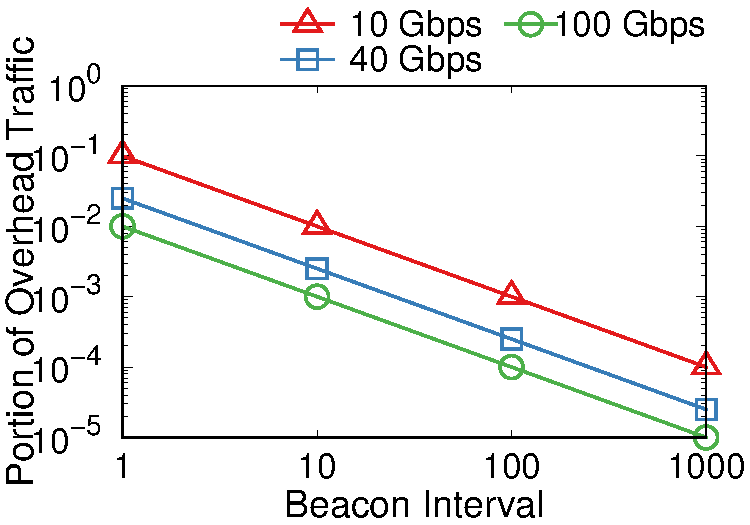
\includegraphics[width=.23\textwidth]{gnuplot/beacon_network_overhead.pdf}}
	\hspace{0.01\textwidth}
	\subfloat[CPU processing overhead.\label{fig:cpu-overhead}]
	{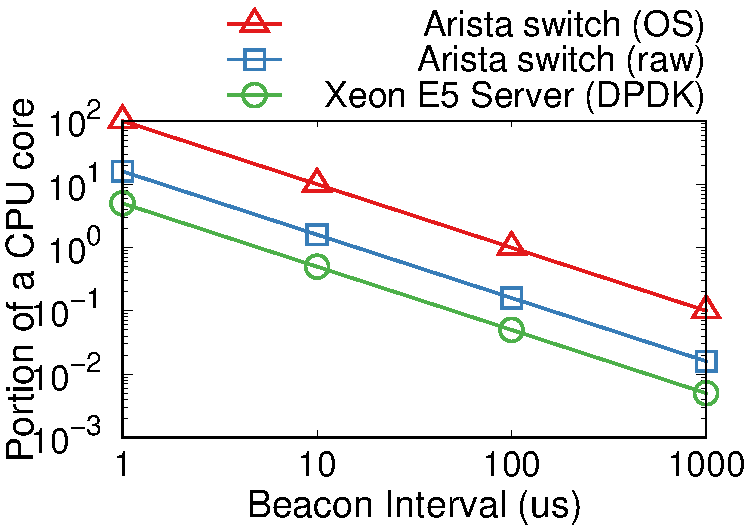
\includegraphics[width=.23\textwidth]{gnuplot/beacon_cpu_overhead.pdf}}
	\caption{
		Beacon overhead under different beacon intervals and network throughput.
		CPU processing overhead for Arista switch is extrapolated.
	}
\label{fig:overhead}
\end{figure}


%\begin{figure}[t]
%\centering
%
\includegraphics[width=0.48\textwidth]{images/fixme.pdf}
%\caption{CDF of end-to-end delay and reordering delay.}
%\label{fig:cdf-delay}
%\end{figure}


\subsubsection{Network Overhead}
\label{sec:eval-overhead}


\RED{In the evaluation about beacon overhead, we should not simply show a line chart of reordering delay and beacon overhead. This figure is trivial and should be removed.}

Beacons are network packets that consume bandwidth.
As shown in Figure~\ref{fig:network-overhead}, under high speed networks and a reasonable beacon interval, the beacon traffic is a tiny portion of available link bandwidth.
Because beacons are hop-by-hop, the overhead is only related to beacon interval and does not change with system scale.

\subsubsection{CPU Overhead}
\label{sec:eval-cpu-overhead}

The CPU overhead of \sys has two parts: beacon processing on switches and reordering on receivers.
Figure~\ref{fig:cpu-overhead} shows the number of cores required for beacon processing of a 32-port switch.
The Arista switch has 4 CPU cores.
The raw packet processing capacity of a switch CPU core is 1/3 of a Xeon E5 CPU core.
If we are able to bypass the kernel network stack and process packets efficiently in Arista switches, a single switch CPU core can sustain 10~$\mu$s beacon interval.


\begin{figure}[t]
\centering
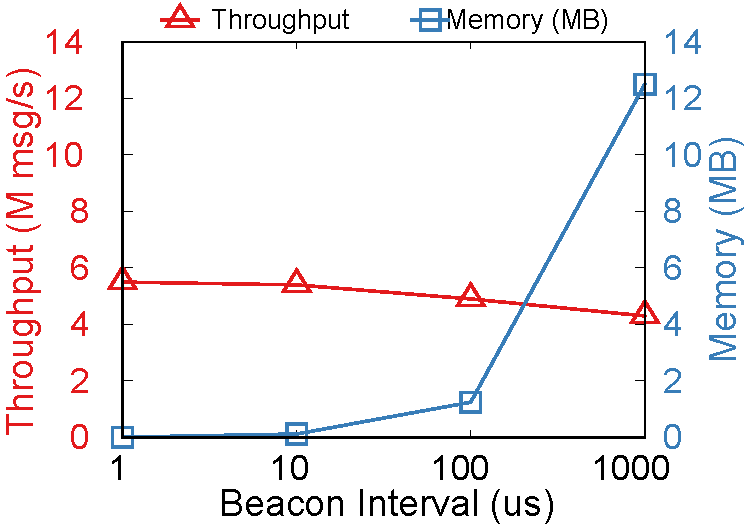
\includegraphics[width=0.3\textwidth]{gnuplot/reorder_receiver.pdf}
\caption{[Testbed] Reordering overhead on receivers.}
\label{fig:reorder-overhead}
\end{figure}

As shown in Figure~\ref{fig:reorder-overhead}, although the maximal buffer size required on the receiver increases linearly with beacon interval, the message reordering throughput of a CPU core does not degrade significantly.

\subsection{Deep Dive}

\begin{table}
\centering
\scalebox{0.9}{
\begin{tabular}{l|r|r|r|r}
	\hline
	 & $S_1 \rightarrow R_1$ & $S_1 \rightarrow R_2$ & $S_2 \rightarrow R_1$ & $S_2 \rightarrow R_2$ \\
    \hline
    \hline
    $S_1$ fail & N/A & N/A & $T_{timeout}$ & $T_{timeout}$ \\
    \hline
    $S_1$ recover & RTT & RTT & 0 & 0 \\
    \hline
    $R_1$ fail & N/A & $T_{timeout}$ & N/A & $T_{timeout}$ \\
    \hline
    $R_1$ recover & RTT & 0 & RTT & 0 \\
    \hline
    $SW_1$ fail & $T_{timeout}$ & $T_{timeout}$ & $T_{timeout}$ & $T_{timeout}$ \\
    \hline
    $SW_1$ recover & 0 & 0 & 0 & 0 \\
    \hline
\end{tabular}
}
\caption{
	Convergence time after failure and recovery of host and switch.
	Convergence time is the time since the event occurs until end-to-end delay recovers to normal.
    Convergence time 0 indicates not affected.
    $T_{timeout}$ is the beacon timeout for failure detection.
}
\label{tab:failure}
\end{table}

We consider a network with two senders $S_1, S_2$, two receivers $R_1, R_2$ interconnected via two switches $SW_1, SW_2$.
Each switch is connected to all four hosts.
Table~\ref{tab:failure} shows how long a failure or recovery would impact the system.
\RED{Bojie will fill the table.}

\iffalse
\subsubsection{Incremental Deployment}
\label{sec:eval-incremental}


\begin{figure}[t]
\centering
	\subfloat[Clock convergence.\label{fig:clock-convergence}]
	{
\includegraphics[width=.23\textwidth]{images/fixme.pdf}}
	\hspace{0.01\textwidth}
	\subfloat[Reordering delay.\label{fig:incremental-delay}]
	{
\includegraphics[width=.23\textwidth]{images/fixme.pdf}}
\caption{[Simulation] Merging two running TOMS systems by adding a network link between them.}
\label{fig:incremental}
\end{figure}

Figure~\ref{fig:clock-convergence} shows
Converge time graph, compare with physical time synchronization solution

Figure~\ref{fig:incremental-delay} shows the reordering delay. (spike then fall back)
\fi



